\section{Reputation}
\label{sec:reputation}

\nemquote{
It takes many good deeds to build a good reputation, and only one bad one to lose it.
}{Benjamin Franklin}

\codenamechapterfirstword uses a peer-to-peer (P2P) network.
P2P networks have the great advantage of being robust because they cannot be shut down by eliminating a single node.
Nevertheless, a public network comes with its own challenges.
The participants of the network are anonymous and anyone can join.
This makes it very easy to inject hostile nodes into the network that spread invalid information or try to disturb the network in some way.

There is a need to identify hostile nodes and reduce communication with them.
There have been many approaches to achieve this.
One of the most successful is building a reputation system for nodes.
\codenamespace follows this approach by implementing simple reputation system.
This chapter will outline the heuristics used.

\subsection{Connection Management}
\index{reputation!connection!management}
\label{sec:reputation:ConnectionManagement}

Each node can establish at most \nemsetting{node}{maxConnections} persistent connections at once.
This limit is expected to be much smaller than the hundreds of thousands of nodes that make up the network as a whole.
In order to avoid isolated node groups from forming, a node will periodically drop existing connections to make room for new connections to different nodes.

When determining the nodes from which to disconnect, a node inspects the ages of all of its connections.
In order to minimize connection overhead, only connections that have been established for at least \nemsetting{node}{maxConnectionAge} rounds are eligible for removal.
The next time a node selection round is done, these connections are dropped and replaced with new connection to other nodes.
This guarantees that over time each node will make connections to many different nodes in the network.

\subsection{Weight Based Node Selection}
\index{reputation!node!selection}
\label{sec:reputation:NodeSelection}

Nodes primarily communicate with each other via the current persistent connections they have established.
A node can query another node for new transactions or blocks, or ask for a list of other nodes with which it has interacted.
Nodes can also voluntarily send data to other nodes.
Each communication between nodes is considered an interaction and each interaction is scored as either successful, neutral or failed.
For example, when a remote node sends new, valid data the interaction is considered successful because it has contributed to the synchronization of the two nodes.
If the remote node has no new data, the interaction is neutral.
Otherwise, the interaction is considered failed.

Each node keeps track of the outcomes of its own interactions with other nodes.
These outcomes are only used locally and not shared with other nodes.
A node's interactions with other nodes influences the partner nodes it selects.
Interaction results are stored for at most one week but reset on node restart.
These results are time-limited to allow nodes that are having transient failures to reestablish themselves as good partners.

When selecting partner nodes, a node first determines a set of candidate nodes.
Each candidate node is assigned a raw weight between 500 and 10000 according to the following criteria:

\begin{itemize}
\item If there were 3 or fewer non-neutral interactions with the remote node, it is given a medium raw weight of 5000.
This gives new nodes a good chance of getting selected.
\item Else let \textit{s} be the number of successful and \textit{f} the number of failed interactions.
Then the raw weight is calculated by the following formula:

\begin{figure}[t!]
	\nemcenterwithcaption{
		\begin{tikzpicture}[scale=1.5]
			\begin{axis}[
					scaled z ticks=false,
					colormap/cool,
					y dir=reverse,
					zlabel style={rotate=-90},
					xlabel = {$\substack{successful\\interactions}$},
					ylabel = {$\substack{failed\\interactions}$},
					zlabel = {$\substack{raw\\node\\weight}$}
				]
				\addplot3[surf, samples=50, domain=0:100, y domain=50:0] {max(500, x * 10000 / (x + 9 * y))};
			\end{axis}
		\end{tikzpicture}
	}{Raw Node Weight}
\end{figure}

\begin{align*}
\mathit{rawWeight} = \max\left(500, \frac{s \cdot 10000}{s + 9 \cdot f}\right)
\end{align*}
\end{itemize}

This formula guarantees that failed interactions rapidly decrease the weight of a remote node and its likelihood of getting selected.
The presence of a minimum score still gives a node with many failures a slight chance for being selected and possibly improving its score with more interactions.

The raw weight is multiplied with a weight multiplier to give the final weight of a node.
For static nodes, the multiplier is 2.
For dynamic nodes, it is 1.
If a node is banned due to consecutive interaction failures (see section \autoref{sec:reputation:NodeBanning}) , the multiplier is decreased by 1.
This ensures that a node does not connect to dynamic banned nodes.
The chance of connecting to static banned nodes is reduced by half.

Removal candidates are determined based on their connection age.
Each removal candidate that will be closed is replaced with a connection to a new node so that the node maintains the desired level of connections.
Finally, for each free slot, a candidate node has a chance of getting selected given by:

\begin{align*}
P(\textrm{node is getting selected}) = \frac{\textit{node weight}}{\sum\limits_{\substack{candidates\\nodes}} \textit{candidate node weight}}
\end{align*}

\subsection{Node Banning}
\index{reputation!node!banning}
\label{sec:reputation:NodeBanning}

In a public network there could be potentially malicious nodes that try to disturb normal processing of the network.
Therefore, if a node considers a remote node malicious, it will prevent connecting to that node and will not accept incoming connections from it.

Banning is applied at node level and is attached to a node's network scoped identifier \nemrefparens{sec:network:discovery}.
A misbehaving node will be immediately banned for a period of \nemsetting{node}{defaultBanDuration}.
Even after a node is no longer actively banned, the local node will remember for some time (\nemsetting{node}{keepAliveDuration}) that the node was behaving badly and treat repeat violations more severely by banning the node for longer time periods up to \nemsetting{node}{maxBanDuration}.
During banning, no connections with the banned node will be established.
After banning has expired, the node is treated like a normal interaction partner again.
There are various scenarios where a remote node will get banned.
The penalties vary based on the cause.

\makeatletter
\setlength{\@fptop}{0pt}
\makeatother
\begin{figure}[H]
	\nemcenterwithcaption{
		\begin{tabular}{|c|c|c|c|c|}
			\hline
			& \makecell{Connection\\closed} & \makecell{Remote\\can\\reconnect} & \makecell{Remote\\can be\\selected} & \makecell{Remote\\can send\\data}\\
			\hline
			\makecell{Consecutive\\interaction\\failures} & No & - & \makecell{Yes Static\\No Dynamic} & Yes\\
			\hline
			\makecell{Invalid\\data} & Yes & No & No & No\\
			\hline
			\makecell{Exceeded\\read rate} & Yes & No & No & No\\
			\hline
			\makecell{Unexpected\\data} & Yes & Yes & \makecell{Yes\\(after reconnect)} & \makecell{Yes\\(after reconnect)}\\
			\hline
		\end{tabular}
	}{Banning Rules}
\end{figure}

\subsubsection*{Consecutive Interaction Failures}
If interactions with the same node fail for too many consecutive times due to networking or stateful failures, it is better to suspend all interactions with that node for some time, hoping the node will behave better in the future.
The number of consecutive interaction failures before the node gets banned can be configured.
The amount of time the node gets banned is measured in selection rounds and can also be configured.
While the node is banned, it will not be actively selected as interaction partner, but it still can send new data.
This violation, therefore, only results in a partial ban.

\subsubsection*{Invalid Data}
Data can be invalid in many ways.
For example, if a remote node is on a fork, it might send a new block that does not fit into the local node's chain.
Little forks with a depth of one or two blocks happen frequently.
Though the sent data is invalid, it is not considered malicious because the remote node's internal state was understandably different.
On the other hand, sending data with invalid signatures clearly indicates that the remote node is malicious because signature verification is independent of a node's state.
The same is true for other verification failures that do not depend on the state of a node.
In all those cases, the remote node gets banned.

\subsubsection*{Exceeded Read Data Rate}
To prevent malicious nodes from spamming other nodes with excessive amounts of data, each node monitors the read rate from the socket used for communication.
If the data read during a configured time interval exceeds a maximum, the socket is closed and the node is banned.
The maximum read rate is configurable.

\subsubsection*{Unexpectedly Receiving Data}
There are situations during node communication where the local node is not expecting to receive any data from the remote.
If the remote still sends data in such a situation, it is violating the protocol and the connection is closed.
In this case, the connection is immediately closed but there is no persistent banning of the node.
